\documentclass[conference]{IEEEtran}
\IEEEoverridecommandlockouts
% The preceding line is only needed to identify funding in the first footnote. If that is unneeded, please comment it out.
\usepackage{cite}
\usepackage{amsmath,amssymb,amsfonts}
\usepackage{algorithmic}
\usepackage{graphicx}
\usepackage{textcomp}
\usepackage{xcolor}
\usepackage{hyperref}
\usepackage{multirow}
\usepackage{colortbl}
\usepackage{caption}
\usepackage{subcaption}
\def\BibTeX{{\rm B\kern-.05em{\sc i\kern-.025em b}\kern-.08em
    T\kern-.1667em\lower.7ex\hbox{E}\kern-.125emX}}

    
\begin{document}

\title{Spla: Generalized Sparse Linear Algebra Library with Vendor-Agnostic GPUs Acceleration\\
\thanks{We would like to thank Huawei Technologies Co., Ltd for supporting this research. We are also grateful to our team and reviewers.\\}}

\author{\IEEEauthorblockN{1\textsuperscript{st} Egor Orachev}
\IEEEauthorblockA{\textit{St. Petersburg State University} \\
St. Petersburg, Russia \\
egor.orachev@gmail.com \\
0000-0002-0424-4059}
\and
\IEEEauthorblockN{2\textsuperscript{nd} Semyon Grigorev}
\IEEEauthorblockA{\textit{St. Petersburg State University} \\
St. Petersburg, Russia \\
s.v.grigoriev@spbu.ru \\
0000-0002-7966-0698}
}

\maketitle

\begin{abstract}
    Scalable high-performance graph analysis is a nontrivial challenge. 
    Usage of sparse linear algebra operations as building blocks for graph analysis algorithms, which is a core idea of GraphBLAS standard, is a promising way to attack it.
    While it is known that sparse linear algebra operations can be efficiently implemented on GPU, full GraphBLAS implementation on GPU is a nontrivial task that is almost solved by GraphBLAST project. 
    It is shown that utilization of GPUs for GraphBLAS implementation significantly improves performance. But GraphBLAST is not portable because it is based on Nvidia Cuda.
    In this work we propose Spla library which aims to solve this problem using OpenCL API for vendor-agnostic GPUs accelerated computations.
    Evaluation shows that the proposed solution demonstrates performance comparable with GraphBLAST, outperforming it up to 36 times in some cases, and remains portable across different GPUs vendors.
\end{abstract}

\begin{IEEEkeywords}
graphs, algorithms, graph analysis, sparse linear algebra, GraphBLAS, GPGPU, OpenCL
\end{IEEEkeywords}

\section{Introduction}

% Commented references
% CuSha~\cite{10.1145/2600212.2600227}
% MapGraph~\cite{10.1145/2621934.2621936/MapGraph}
% Medusa~\cite{6497047/Medusa}
% Gunrock~\cite{7967137}

Scalable high-performance graph analysis is a challenge.
CuSha~\cite{10.1145/2600212.2600227} and Gunrock~\cite{7967137} show that the utilization of GPUs can improve the performance of graph analysis. But the low flexibility and high complexity of API are problems of these solutions. 
A linear algebra based model, formalized in GraphBLAS~\cite{7761646}, provides a user-friendly API. 
While the reference CPU-based implementation for this API, SuiteSparse~\cite{10.1145/3322125}, demonstrates good performance on real-world tasks, GPU-based implementation is challenging due to required operations generalization, data sparsity, and hardware programming complexity. 
Such well-known libraries as cuSPARSE, clSPARSE, bhSPARSE cannot be reused, since almost all of them are specified for operations over floats. 
GraphBLAST~\cite{yang2019graphblast} and GBTL~\cite{7529957} show promising GPU performance of GraphBLAS-based graph analysis solutions. 
But these solutions are not portable because they are based on Nvidia Cuda. 
Portable solution is a challenge due to intricate GPU programming. 
To address this problem, we developed the GraphBLAS-inspired \textit{Spla\footnote{Source code and project page: \url{github.com/SparseLinearAlgebra/spla}}} library, which features portable OpenCL-based acceleration and shows performance comparable with GraphBLAST, achieving speedup of up to 36 times.
\section{Proposed Solution}

The proposed Spla library implemented in C++17 language, using vendor-agnostic OpenCL 1.2 for GPU specific computations. The OpenCL is chosen over Cuda and SyCL technologies. While Cuda is specific only for Nvidia devices, SyCL is a promising API, but it is too high-level and its support is still debatable. The implementation of linear algebra operations is based on Yang et al.~\cite{7284398:spvspm, https://doi.org/10.48550/arxiv.1804.03327:pushpull, yang2019graphblast} works. Common graph algorithms, such as BFS, SSSP, PR and TC implemented with respect to GraphBLAST. Spla features a number of optimizations, such as push-pull, masking, early exit, custom small memory allocation, and sparse-dense storage switch.
\section{Evaluation}

For performance analysis of the proposed solution, we evaluated a few most common graph algorithms using real-world sparse matrix data. 
As a baseline for comparison we chose LAGraph~\cite{szarnyas2021lagraph} in connection with SuiteSparse~\cite{10.1145/3322125} as a multi-core CPU tool, Gunrock~\cite{7967137} and GraphBLAST~\cite{yang2019graphblast} as a Nvidia GPU tools. 
Also, we tested algorithms on several devices with distinct OpenCL vendors in order to validate the portability of the proposed solution. 

\subsection{Evaluation Setup}

We use a PC with Ubuntu 20.04 installed, which has 3.40Hz Intel Core i7-6700 4-core CPU, DDR4 64Gb RAM, either Nvidia GeForce GTX 1070 8Gb VRAM, Intel Arc A770 flux 8GB VRAM, or AMD Radeon Vega Frontier Edition, 16GB VRAM. Programs were compiled with GCC v9.4. Programs using CUDA were compiled with GCC v8.4 and Nvidia NVCC v10.1.
Data loading time, preparation, format transformations, and host-device initial communications are excluded from time measurements. 
All tests are averaged across 10 runs. 
The deviation of measurements does not exceed the threshold of 10 percent. 
Additional warm-up run is excluded from measurements. 
The 1st graph vertex is initial node in traversal algorithms.

Thirteen matrices with graph data were selected from the Sparse Matrix Collection at University of Florida~\cite{dataset:10.1145/2049662.2049663}. 
Information is summarized in Table~\ref{dataset:info}. 
The dataset is converted to undirected graphs. 
Self-loops and duplicated edges are removed. 
Weights generated using uniform distribution $[0, 1]$ of floating-point values.
 
\begin{table}[tbp]
\caption{Dataset description.} 
\begin{center}
    \scalebox{0.8}{
    \begin{tabular}{|l|r|r|r|r|r|}
    \hline
    \multirow{2}{*}{Graph} & \multirow{2}{*}{Vertices} & \multirow{2}{*}{Edges} & \multicolumn{3}{c|}{Out Degree} \\ 
    \cline{4-6} & & & \multicolumn{1}{r|}{Avg} & \multicolumn{1}{r|}{Sd} & \multicolumn{1}{r|}{Max} \\
    \hline
    \hline
    \rowcolor{black!10} coAuthorsCit&227.3K&1.6M&7.2&10.6&1.4K\\
    \rowcolor{black!2 } coPapersDBLP&540.5K&30.5M&56.4&66.2&3.3K\\
    \rowcolor{black!10} amazon2008&735.3K&7.0M&9.6&7.6&1.1K\\
    \rowcolor{black!2 } hollywood2009&1.1M&112.8M&98.9&271.9&11.5K\\
    \rowcolor{black!10} comOrkut&3.1M&234.4M&76.3&154.8&33.3K\\
    \rowcolor{black!2 } citPatents&3.8M&33.0M&8.8&10.5&793.0\\
    \rowcolor{black!10} socLiveJournal&4.8M&85.7M&17.7&52.0&20.3K\\
    \rowcolor{black!2 } indochina2004&7.4M&302.0M&40.7&329.6&256.4K\\
    \hline
    \rowcolor{black!10} belgiumosm&1.4M&3.1M&2.2&0.5&10.0\\
    \rowcolor{black!2 } roadNetCA&2.0M&5.5M&2.8&1.0&12.0\\
    \rowcolor{black!10} rggn222s0&4.2M&60.7M&14.5&3.8&36.0\\
    \rowcolor{black!2 } rggn223s0&8.4M&127.0M&15.1&3.9&40.0\\
    \rowcolor{black!10} roadcentral&14.1M&33.9M&2.4&0.9&8.0\\
    \hline
    \end{tabular}
    }
    \label{dataset:info}
\end{center}
\end{table}

\subsection{Results Summary}

\begin{figure}[tbp]
\centering
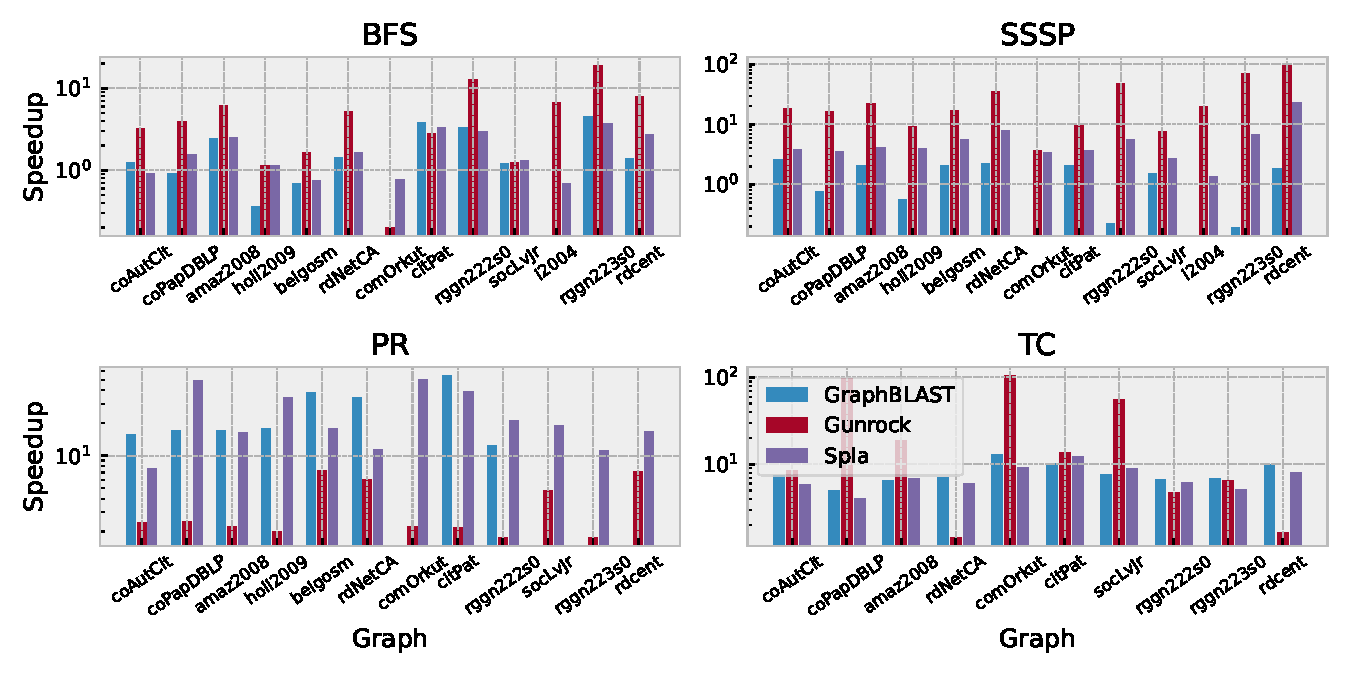
\includegraphics[width=1.0\linewidth]{plots/rq1_rel.pdf}
\caption{Performance of Spla library and GPU tools on the same device, shown as a speedup relative to LaGraph. Logarithmic scale is used.}
\label{fig:rq1_chart}
\end{figure}

\begin{figure}[tbp]
\centering
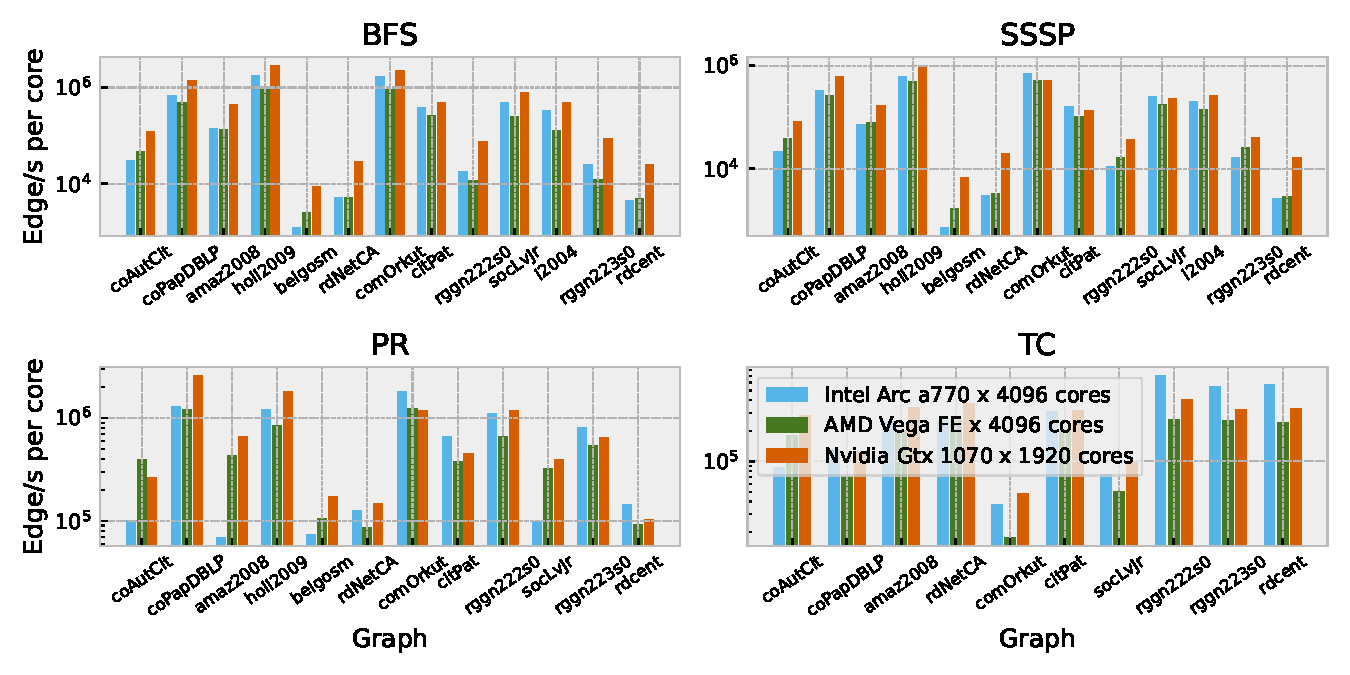
\includegraphics[width=1.0\linewidth]{plots/rq2_cores.pdf}
\caption{Performance of Spla library on different devices, shwon as edge/s througput per device core. Logarithmic scale is used.}
\label{fig:rq2_chart}
\end{figure}

\textbf{RQ1.} \textit{What is the performance of the proposed solution relative to existing tools for GPU analysis?} Taking a look at Fig.~\ref{fig:rq1_chart}, Spla shows very acceptable performance in all algorithms, running with comparable speed to its nearest competitor, GraphBLAST. Also proposed library does not suffer from memory issues on some large graphs. Spla is consistently several times faster than LaGraph, overcoming it up to $25\times$ in some cases. Gunrock is the fastest GPU framework for analysis. It dominates the overall performance and only suffers in a PR algorithm.\\

\textbf{RQ2.} \textit{What is the performance of the proposed solution on various devices vendors and OpenCL runtimes?} Spla successfully launches and workes on the GPU of distinct vendors, including Intel, AMD and Nvidia. It shows promising performance and demonstrated scalability in relation to the number of computing cores. Fig.~\ref{fig:rq2_chart} depicts the edge/s throughput per a GPU core for all devices. This metric is quite predictable for the same graphs. This can be seen if one takes into account the overall shape of the figures for BFS, SSSP and PR as a whole.
\chapter*{Conclusion}                       % Заголовок
\addcontentsline{toc}{chapter}{Conclusion}  % Добавляем его в оглавление

%% Согласно ГОСТ Р 7.0.11-2011:
%% 5.3.3 В заключении диссертации излагают итоги выполненного исследования, рекомендации, перспективы дальнейшей разработки темы.
%% 9.2.3 В заключении автореферата диссертации излагают итоги данного исследования, рекомендации и перспективы дальнейшей разработки темы.

\begin{enumerate}[beginpenalty=10000] % https://tex.stackexchange.com/a/476052/104425
	\item Разработан подход к поиску путей в графе с заданными КС-ограничениями на основе методов линейной алгебры, который позволяет использовать теоретические и практические достижения линейной алгебры для решения данной задачи.
	\item Разработан алгоритм, использующий предложенный подход и решающий задачи поиска путей в графе с заданными КС-ограничениями. Доказана завершаемость и корректность предложенного алгоритма. Получена теоретическая оценка сверху временной сложности алгоритма. Предложенный алгоритм использует операции над матрицами, которые позволяют применять широкий класс оптимизаций и дают возможность автоматически распараллеливать вычисления за счёт существующих библиотек линейной алгебры.
	\item Разработан алгоритм поиска путей в графе с заданными КС-ограничениями, использующий предложенный подход и не требующий преобразования входной КС-грамматики. Доказана завершаемость и корректность предложенного алгоритма. Получена теоретическая оценка сверху временной сложности алгоритма. Предложенный алгоритм позволяет работать с произвольными входными КС-грамматиками без необходимости их преобразования, что позволяет избежать значительного увеличения размеров входной грамматики и увлечения времени работы алгоритма.
	\item Предложенные алгоритмы реализованы с использованием параллельных вычислений. Проведено экспериментальное исследование разработанных алгоритмов на реальных RDF данных и графах, построенных для статического анализа программ. Было проведено сравнение полученных реализаций между собой, с существующими решениями из области статического анализа и с решениями, основанными на различных алгоритмах синтаксического анализа. Результаты сравнения показывают, что предложенные реализации для задачи достижимости позволяют ускорить время анализа до 2 порядков и потребляют до 2 раз меньше памяти по сравнению с существующими решениями, а для задач поиска одного и поиска всех путей в графе позволяют ускорить время анализа до 3 порядков и до 2 порядков снизить потребление памяти.
\end{enumerate}


$\textit{CFPQ\_PyAlgo}$ platform for developing, testing, and benchmarking CFPQ algorithm was created using the obtained implementations.

We give the following \textbf{application recommendations for the work results}. The developed approach and the obtained algorithms are applicable for the CFPQ using linear algebra. Also, provided approach allows one to obtain high-performance parallel CFPQ implementations that are compact and portable. These implementations can be created using existing linear algebra libraries. The $\textit{CFPQ\_PyAlgo}$ platform can be used in static program analysis~\cite{rehof2001type,zheng2008demand}, RDF analysis~\cite{zhang2016context}, bioinformatics~\cite{sevon2008subgraph}, etc. In addition, CFPQ implementations can be integrated with graph databases such as RedisGraph. In work~\cite{azimov2}, we provided such prototype implementations. However, to provide full integration it is necessary to extend Cypher graph query language used in RedisGraph and to support syntax for specification of context-free path constraints. Moreover, there is a proposal$\footnote{A proposal with path pattern syntax for openCypher:\\ https://github.com/thobe/openCypher/blob/rpq/cip/1.accepted/CIP2017-02-06-Path-Patterns.adoc (date of access: 14.01.2022).}$ that describes such syntax extension.

Also, we identify \textbf{prospects for further development of the topic}. First of all, the proposed approach and developed algorithms can be applied to creation of a specialized tool for a specific graph analysis problem. The CFPQ algorithms for graphs of a certain type and for specific path constraints can be created using the proposed approach. For example, for a static program analysis the structure of graphs derived from programs in a particular programming language can be taken into account, as well as the properties of a particular CFL for the chosen analysis (alias analysis~\cite{zheng2008demand}, taint analysis~\cite{taint}, etc.).

In practice, CFPQ problem is rarely solved without fixing a relatively small set of possible source and destination vertices. Thus, often the information about paths between any vertices is redundant. Therefore, another direction of further research is modification of all proposed CFPQ algorithms with additional restrictions on sets of source and destination vertices.

In this work, the proposed matrix-based CFPQ algorithm for the single-path and all-path query semantics was implemented only on CPU. For these query semantics, we use more complex data types for matrix elements. This leads to a significant increase in memory consumption and does not allow us to obtain a high-performance GPU implementation. Therefore, further research is needed to optimize this algorithm and the algebraic structures used. In the future, it may be possible to obtain high-performance GPU implementations of this algorithm using the CUSP library and the GraphBLAST library.

In addition, there are some graph analysis problems that cannot be expressed using the context-free path constraints. For example, the context-sensitive data-dependence program analysis~\cite{linearconjunctive} uses an interleaved matched-parenthesis language that is not context-free. This problem is well-known to be undecidable~\cite{linearconjunctive}. However, path constraints in the form of linear conjunctive languages~\cite{okhotin2001conjunctive} that belong to a wider class of languages than context-free ones, can be used to approximate the result of such analysis. Thus, the relevant research direction is to extend the proposed approach to solve path querying problems with path constraints expressed by languages from a broader class of languages than the CFLs.


\bibliographystyle{IEEEtran}
\bibliography{spla_hpec}

\end{document}
